\newpage
{\bfseries IRSTI 50.41.29};14.01.85

\sectionwithauthors{K.Akishev, A.Тulegulov, D. Zhamangarin, Z.Nurtai, E. Ospanov}{EVALUATION OF THE EFFECTIVENESS OF USING THE SOFTWARE PRODUCT
"ASSISTANT FOR THE PREPARATION OF TEST TASKS" TO TEST THE KNOWLEDGE OF
STUDENTS}

\begin{center}
{\bfseries \textsuperscript{1}K.Akishev\textsuperscript{🖂},\textsuperscript{1}A.Тulegulov,
\textsuperscript{1}D. Zhamangarin , \textsuperscript{1}Z.Nurtai,
\textsuperscript{2}E. Ospanov}

\textsuperscript{1}Kazakh University of Technology and Business named
after K.Kulazhanov, Astana, Kazakhstan,

\textsuperscript{2}NJSC ''Shakarim University'', Semey, Kazakhstan

Corresponding author:\emph{Akmail04cx@mail.ru}
\end{center}


The educational and methodological set of documentation (UMKD) is an
integral part of the educational process at a higher educational
institution.

One of the types of control of a student at a higher educational
institution is passing a test. Currently, it is the most common and
popular tool used in many disciplines, providing a transparent, fast and
quite practical way of verifying students\textquotesingle{} knowledge.

When developing tests, teachers use various programs, while spending
quite a lot of time to prepare, first, control questions, and then add
them to the appropriate program.

In this regard, the purpose of our research is the need to develop
software code that allows you to use ChatGPT for the automated formation
of test tasks when checking the knowledge of students.

The developed computer program "Assistant for the preparation of test
tasks" allows you to automate the process of preparing test tasks for
text of any volume and number of questions;

The program code can be used in educational institutions of the Ministry
of Education and the Ministry of Science and Higher Education of the
Republic of Kazakhstan.

The practical application of the developed program "Assistant for the
preparation of test tasks" allows to increase the effectiveness of the
teacher\textquotesingle s work by 80\% compared to existing analogues
for the development of test tasks. At the same time, the quality and
adequacy of the developed issues are at a high level.

{\bfseries Key words}: automation, information technology, software
product, test tasks, efficiency, student.

\begin{center}

{\bfseries БІЛІМ АЛУШЫЛАРДЫҢ БІЛІМІН ТЕКСЕРУ ҮШІН "ТЕСТ ТАПСЫРМАЛАРЫН
ДАЙЫНДАУ КӨМЕКШІСІ" БАҒДАРЛАМАЛЫҚ ӨНІМІН ПАЙДАЛАНУ}

{\bfseries ТИІМДІЛІГІН БАҒАЛАУ}

{\bfseries \textsuperscript{1}К.Акишев\textsuperscript{🖂},
\textsuperscript{1}А.Тулегулов, \textsuperscript{1}Д. Жамангарин,
\textsuperscript{1}Ж.Нұртай, \textsuperscript{2}Е.Oспанов}

\textsuperscript{1}Қ.Құлажанов атындағыҚазақ технология және бизнес
университеті АҚ, Астана, Казахстан ,

\textsuperscript{2}Шакарим атындағы университет КЕАҚ, Семей, Қазақстан,

е-mail:Akmail04cx@mail.ru
\end{center}

Құжаттаманың оқу-әдістемелік жиынтығы (ОӘК) жоғары оқу орнындағы оқу
процесінің ажырамас бөлігі болып табылады.

Жоғары оқу орнында білім алушыны бақылаудың бір түрі-тест тапсыру.
Қазіргі уақытта бұл көптеген пәндер бойынша қолданылатын ең кең таралған
және танымал құрал, білім алушылардың білімін тексерудің мөлдір, жылдам
және практикалық түрін қамтамасыз етеді.

Тесттерді әзірлеу кезінде мұғалімдер әртүрлі бағдарламаларды
пайдаланады, ал алдымен тест сұрақтарын дайындауға, содан кейін оларды
тиісті бағдарламаға енгізуге жеткілікті уақыт ресурстары жұмсалады.

Осыған байланысты, біздің зерттеуіміздің мақсаты білім алушылардың
білімін тексеру кезінде тест тапсырмаларын автоматтандырылған
қалыптастыру үшін chatgpt пайдалануға мүмкіндік беретін бағдарламалық
кодты әзірлеу қажеттілігі болып табылады.

"Тест тапсырмаларын дайындау көмекшісі" компьютеріне арналған әзірленген
бағдарлама тест тапсырмаларын дайындау процесін автоматтандыруға
мүмкіндік береді, кез-келген көлемдегі мәтін мен сұрақтар саны үшін;

Бағдарламалық код Қазақстан Республикасы Білім министрлігі мен ғылым
және жоғары білім министрлігінің Білім беру мекемелерінде пайдаланылуы
мүмкін.

Әзірленген "тест тапсырмаларын дайындау көмекшісі" бағдарламасын
практикалық қолдану тест тапсырмаларын әзірлеу үшін қолданыстағы
аналогтармен салыстырғанда оқытушының жұмыс тиімділігін 80\% - ға
арттыруға мүмкіндік береді. Бұл ретте әзірленген мәселелердің сапасы мен
барабарлығы жоғары деңгейде.

{\bfseries Түйін сөздер}: автоматтандыру, ақпараттық технологиялар,
бағдарламалық өнім, тест тапсырмалары, тиімділік, білім алушы
\begin{center}

{\bfseries ОЦЕНКА ЭФФЕКТИВНОСТИ ИСПОЛЬЗОВАНИЯ ПРОГРАММНОГО ПРОДУКТА
«ПОМОЩНИК ПОДГОТОВКИ ТЕСТОВЫХ ЗАДАНИЙ» ДЛЯ ПРОВЕРКИ ЗНАНИЙ ОБУЧАЮЩИХСЯ}

{\bfseries \textsuperscript{1}К.Акишев\textsuperscript{🖂},
\textsuperscript{1}А.Тулегулов, \textsuperscript{1}D.Zamangarin,
\textsuperscript{1}Ж. Нуртай, \textsuperscript{2}Е.Oспанов}

\textsuperscript{1}Казахский университет технологии и бизнеса
им.К.Кулажанова, Астана, Казахстан,

\textsuperscript{2} НАО Университет Шакарима, Семей,Казахстан,

е-mail: Akmail04cx@mail.ru
\end{center}

Учебно-методический комплект документации (УМКД), является неотъемлемой
частью учебного процесса в высшем учебном заведении.

Одним из видов контроля обучающегося в высшем учебном заведении является
прохождение теста. В настоящее время --это наиболее распространенный и
популярный инструмент? используемый по многим дисциплинам,
обеспечивающий, прозрачный, быстрый и довольно практичный вид проверки
знаний обучающихся.

При разработке тестов преподаватели используют различные программы, при
этом тратится довольно большой ресурс времени, чтобы подготовить,
сначала контрольные вопросы, а затем внести их в соответствующую
программу.

В этой связи, цель нашего исследования заключается в необходимости
разработки программного кода позволяющего, использовать ChatGPT, для
автоматизированного формирования тестовых заданий, при проверки знаний
обучающихся.

Разработанная программа для ЭВМ «Помощник подготовки тестовых заданий»
позволяет автоматизировать процесс подготовки тестовых заданий, для
текста любого объема и количества вопросов;

Программный код может быть использован в образовательных учреждениях
министерства образования и министерства науки и высшего образования
Республики Казахстан.

Практическое применение разработанной программы «Помощник подготовки
тестовых заданий» позволяет повысить эффективность работы преподавателя
на 80\% по сравнению с существующими аналогами для разработки тестовых
заданий. При этом качество и адекватность разработанных тестовых
вопросов на высоком уровне.

{\bfseries Ключевые слова}: автоматизация, информационные технологии,
программный продукт, тестовые задания, эффективность, обучающийся

\begin{multicols}{2}

{\bfseries Introduction.} The adoption of the Law on Digitalization in the
Republic of Kazakhstan {[}1{]} requires the use of information
technology achievements in all sectors of the economy, including in the
field of education {[}2{]}.

It should be understood that the effectiveness of obtaining high-quality
education ensures objective control of students\textquotesingle{}
knowledge and skills. In practice, two types of control are used --
subjective and objective. The first one is characterized by the personal
ideas of the examiner in relation to the student. And in practice, it
may not always be objective, for a number of reasons, including the
teacher\textquotesingle s likes and dislikes for the student. As for the
second type of control, which is now used both in schools and in higher
educational institutions, they include a criterion-oriented test, which
serves as a measure of the quality of learning by students.

If we ask ourselves why testing has become so widely used, then we get
the answer:

1) a more adequate and reliable method that allows students to be put on
an equal footing;

2) mobilizes the work of the brain in conditions of maximum
concentration and responsibility;

3) Excludes human influence.

One of the main criteria of software products used for test control is
saving time, as well as time spent on developing software code.

Although the material costs associated with the use of testing are much
higher from the point of view of the organization, but the efficiency is
much higher.


Table 1 shows the most common test development programs.
\end{multicols}


{\bfseries Table 1−Test development programs}

\begin{longtable}[]{@{}
  >{\raggedright\arraybackslash}p{(\columnwidth - 2\tabcolsep) * \real{0.3137}}
  >{\raggedright\arraybackslash}p{(\columnwidth - 2\tabcolsep) * \real{0.6863}}@{}}
\toprule\noalign{}
\begin{minipage}[b]{\linewidth}\raggedright
Title
\end{minipage} & \begin{minipage}[b]{\linewidth}\raggedright
Functional
\end{minipage} \\
\midrule\noalign{}
\endhead
\bottomrule\noalign{}
\endlastfoot
TestMaker & -editing previously created tests;

-save test results;

-adding graphic images;

-Generate questions in random order. \\
RichTest & Differs from the previous one by the possibility of:

-transition to theory to prepare for the test;

- setting the difficulty of each question;

- attaching a hint to a question

- the user switches to the training mode. \\
Examiner & Practically no different from TestMaker \\
MyTestXPro & The difference from the previous ones:

-single selection;

-multiple choice;

-establishment of the order of succession;

-establishing compliance;

-indication of the truth or falsity of statements; \\
INDIGO & Features:

-tasks for each group of individual settings. \\
\end{longtable}

\begin{multicols}{2}


The disadvantages of the above programs are the need for manual
formation of questions, considerable time for the development of tests.

In this regard, there is a problem in the need to automate the
preparation of test tasks while maintaining the quality of the
questions, the ability to edit, the availability of adequate ergonomics
and use for mobile applications.

The purpose of the study: The development of software code that allows
you to automate the process of preparing test tasks using ChatGPT
capabilities.

{\bfseries Materials and methods.} The computer program "Assistant for
preparing test tasks" was developed using JavaScript, HTML, CSS to
create HTTP requests and interact with the ChatGPT API.

{\bfseries Discussion of the results.} The development of the program code
begins with going to the project folder and http://localhost:3000 we
will launch the development server.
\end{multicols}


{\bfseries Open the file located at the address (see fig.1)}
\begin{figure}[H]
	\centering
	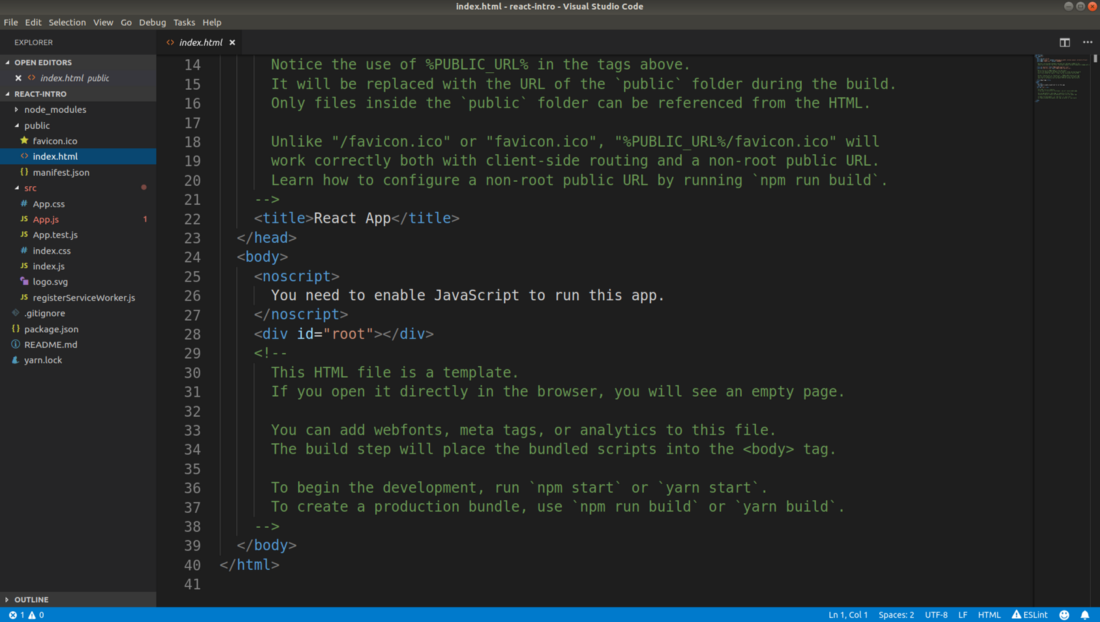
\includegraphics[width=0.8\textwidth]{assets/126}
	\caption*{\bfseries Figure 1− Index.html files}
\end{figure}
\begin{multicols}{2}

Our React application will be placed in the \textless div
id="root"\textgreater{} line. The element will be replaced with the
application code, and everything else will remain the same.

Open the src / index js file, the React application is located here, the
source code of the application is located in the src directory (see fig.
2).

Let\textquotesingle s look at the code of our first component. Src / App (see fig. 3). 
\end{multicols}


\begin{figure}[H]
	\centering
	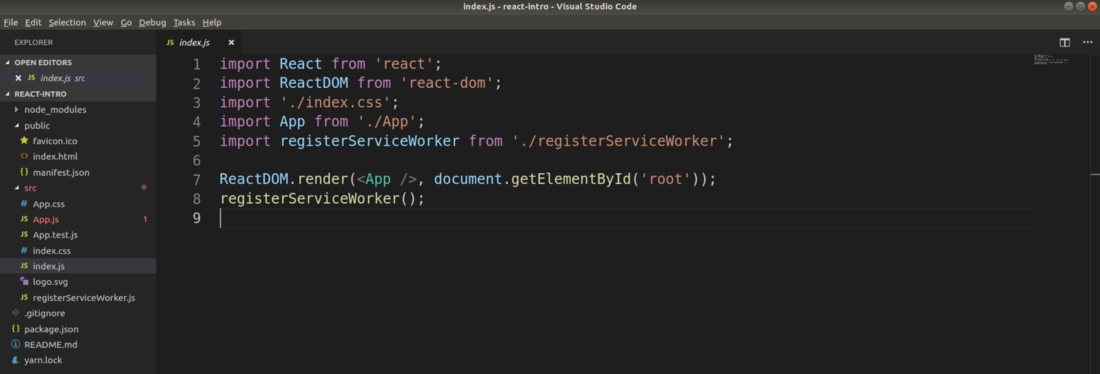
\includegraphics[width=0.8\textwidth]{assets/127}
	\caption*{\bfseries Figure 2−Index.js files}
\end{figure}


\begin{figure}[H]
	\centering
	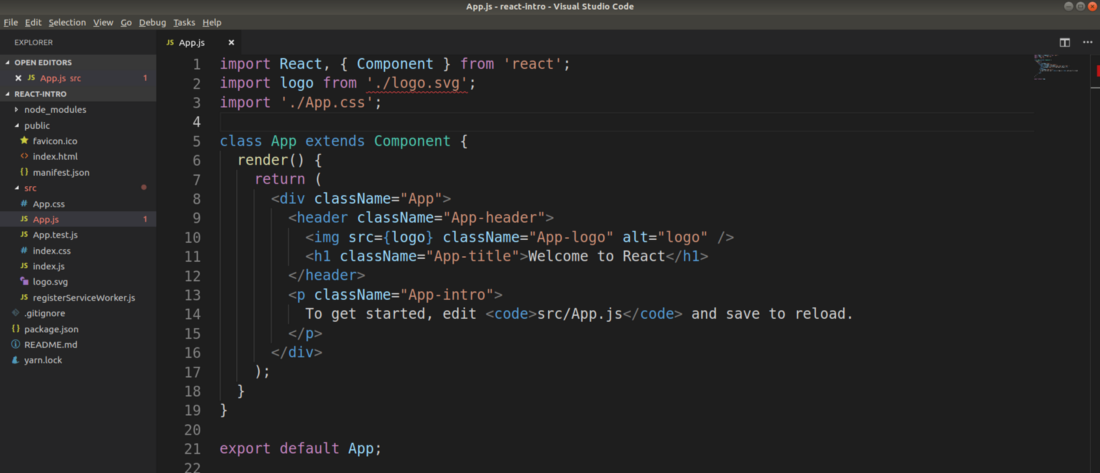
\includegraphics[width=0.8\textwidth]{assets/128}
	\caption*{\bfseries Figure 3− App.js files}
\end{figure}

\begin{multicols}{2}

Let\textquotesingle s consider the principle of using ChatGPT in our
study.

By creating HTTP API requests, we can interact with ChatGPT and receive
responses in real time {[}3-8{]}.

This requires tools and accounts in particular:

-\/-Open ID account and API key (registering an account on the Open AI
platform and obtaining an API key to authenticate ChatGPT API requests;

-the presence of a Node.js and npm;

-a project in the React JS Project.

The next important point is to create a component to control the chat
function (see listing 1 of the program code).The program is written
using the Russian alphabet.

Listing 1 of the program code:
\end{multicols}


// Chat.js

Import React , \{ useState \} внутринний
\textquotesingle react\textquotesingle{} ;

аксиомы \textquotesingle axios\textquotesingle{} внутрениий импорт;

const чат = () =\textgreater{} \{

const {[}input, setInput{]} = useState
(\textquotesingle\textquotesingle);

const {[}известия, setMessages{]} = useState({[}{]});

const sendMessage = async() =\textgreater{} \{

он бір

if (вход. Trim () === \textquotesingle\textquotesingle) возвращение;

// ChatGPT API-ге выполните запрос

попытка \{

const ответ = аксиома ожидание. почты (

\textquotesingle https://api.openai.com/v1/engines/davinci-codex/completions\textquotesingle{}
,

\{

определение: ввод,

максимальное\_символов: 150,

\},

\{

темы: \{

"Тип контента ": "application/json"

\textquotesingle Авторизация\textquotesingle{} : \textquotesingle Media
\$\{ процесс . конв. REACT\_APP\_OPENAI\_API\_KEY \}`

\},

\}

);

// Обновите Статус, используя ответ

тридцать

setMessages ({[} ... сообщение , \{ текст : ввод , тип :
\textquotesingle пользователь\textquotesingle{} \}{]});

setMessages ({[} ... сообщение , \{ текст : ответ .выбор данных {[} 0
{]}. текст , тип: \textquotesingle месяц\textquotesingle{} \}{]});

setInput(\textquotesingle\textquotesingle);

\} catch (ошибка) \{

консоль error(\textquotesingle\textquotesingle Ошибка отправки сообщения
:\textquotesingle, ошибка);

\}

\};

выход (

\textless ситуация \textgreater{}

\textless ситуация \textgreater{}

\{Карта сообщений(( сообщение , индекс ) =\textgreater{} (

\textless div ключ = \{индекс\} className = \{сообщение. \}
\textgreater введите

\{ информация . тип \}

\textless/del\textgreater{}

))\}

\textless/del\textgreater{}

\textless случай\textgreater{}

\textless тип ввода = «тип»

мән = \{ввод\}

onChange = \{( e ) =\textgreater{} setInput ( например. задача .
значение )\}

Заполните = "Введите сообщение..."

/\textgreater{}

\textless{} button onClick = \{ sendMessage \}
\textgreater Отправить\textless/button\textgreater\hspace{0pt}

\textless/del\textgreater{}

\textless/del\textgreater{}

);

\};

\begin{multicols}{2}

Open AI Chatbot API Node.js provides developers with a framework for
creating intelligent interactive web applications {[}9-12{]}.

Let\textquotesingle s consider a request to the server and create a
download verification component and consider all this using React Hooks.

Let\textquotesingle s create a new React: os create-rect-top
rect-axios-table project.

Follow the link: cd react-axios-table

We use an array of objects as data for our project (see listing 2 of the
program code).

Listing 2 of the program code:

\end{multicols}

{[}

\{

id: 101,

firstName: \textquotesingle Sue\textquotesingle,

lastName: \textquotesingle Corson\textquotesingle,

email: \textquotesingle DWhalley@in.gov\textquotesingle,

phone: \textquotesingle(612)211-6296\textquotesingle,

address: \{

streetAddress: \textquotesingle9792 Mattis Ct\textquotesingle,

city: \textquotesingle Waukesha\textquotesingle,

state: \textquotesingle WI\textquotesingle,

zip: \textquotesingle22178\textquotesingle{}

\},

description: \textquotesingle et lacus magna dolor...\textquotesingle,

\}

{]}

\begin{multicols}{2}


Importing axioms into a component that sends requests to the server:
import axios from \textquotesingle axis\textquotesingle{} in the project
we use React Hooks, useState and import useEffect.

Adding the following code to the component: function App() \{ (see
listing 3 of the program code).

Listing 3 of the program code:
\end{multicols}



const {[}appState, setAppState{]} = useState();

useEffect(() =\textgreater{} \{

const apiUrl =
\textquotesingle http://www.filltext.com/?rows=32\&id=\{number\textbar1000\}\&firstName=\{firstName\}\&lastName=\{lastName\}\&email=\{email\}\&phone=\{phone\textbar(xxx)xxx-xx-xx\}\&address=\{addressObject\}\&description=\{lorem\textbar32\}\textquotesingle;

axios.get(apiUrl).then((resp) =\textgreater{} \{

const allPersons = resp.data;

setAppState(allPersons);

\});

\}, {[}setAppState{]});

return (

\textless div className="app"\textgreater{}

\textless/div\textgreater{}

);

\}

export default App;

\begin{multicols}{2}

The above code checks isLoading when data is loaded and shows a loading
message, if isLoading is erroneous, it is returned.

Let\textquotesingle s consider the description of the program code
"Assistant for preparing test tasks". Fig. 4 shows the entrance to the
program {[}13{]}.
\end{multicols}


\begin{figure}[H]
	\centering
	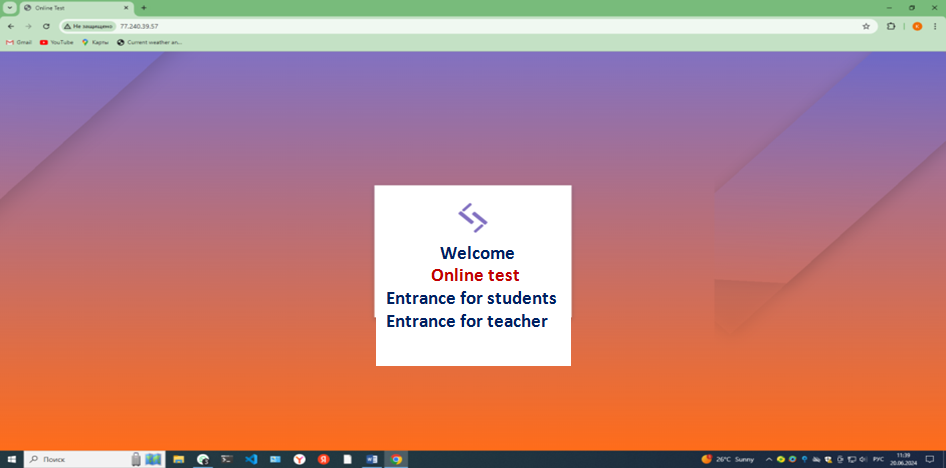
\includegraphics[width=0.8\textwidth]{assets/129}
	\caption*{\bfseries Figure 4−Login to the program}
\end{figure}
\begin{multicols}{2}

The user can log in as a teacher with admin rights, or as a student fig.
5;6.
\end{multicols}

\begin{figure}[H]
	\centering
	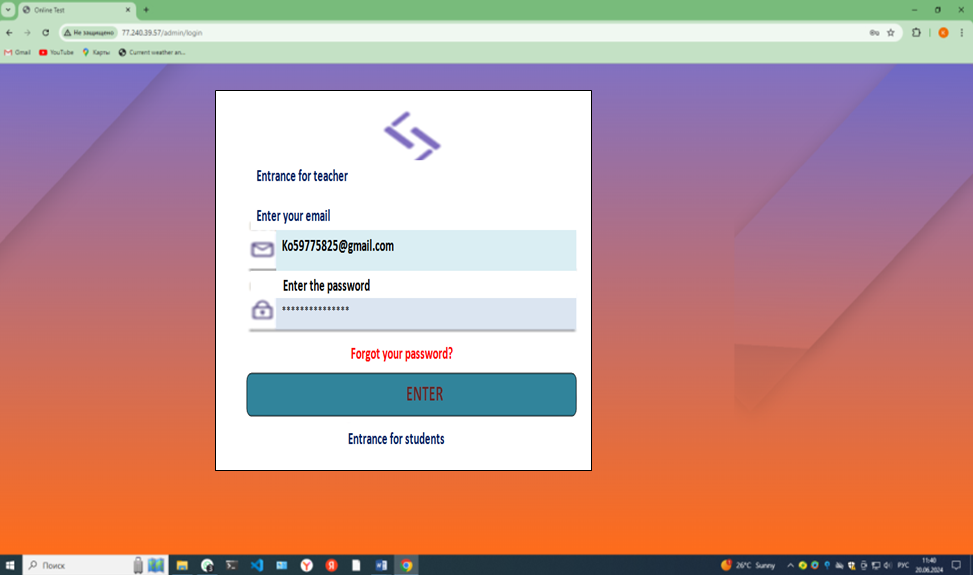
\includegraphics[width=0.8\textwidth]{assets/130}
	\caption*{\bfseries Figure 5−Entering the program as a teacher}
\end{figure}


\begin{figure}[H]
	\centering
	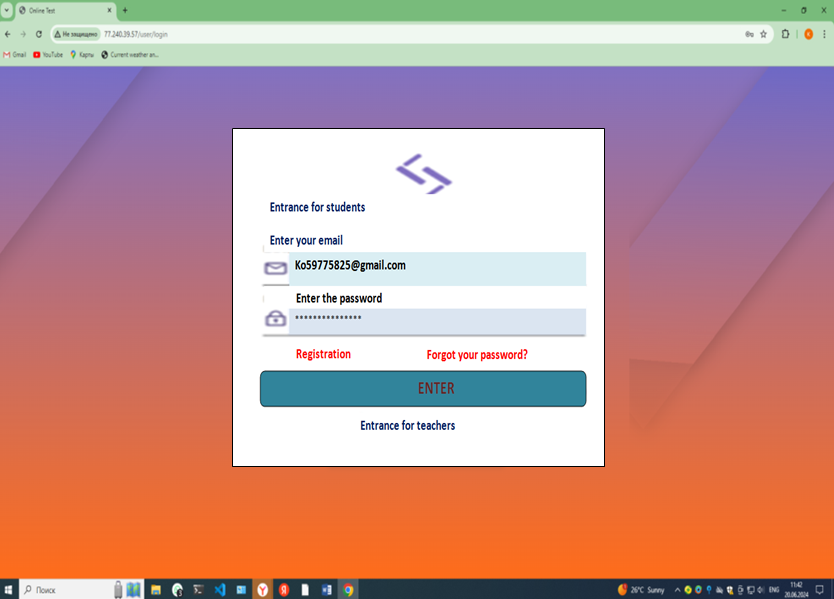
\includegraphics[width=0.8\textwidth]{assets/131}
	\caption*{\bfseries Figure 6−Entering the program as a student}
\end{figure}
\begin{multicols}{2}

The presented software product on the main page contains educational
programs in the disciplines for which it is supposed to develop tests
fig.7.
\end{multicols}

\begin{figure}[H]
	\centering
	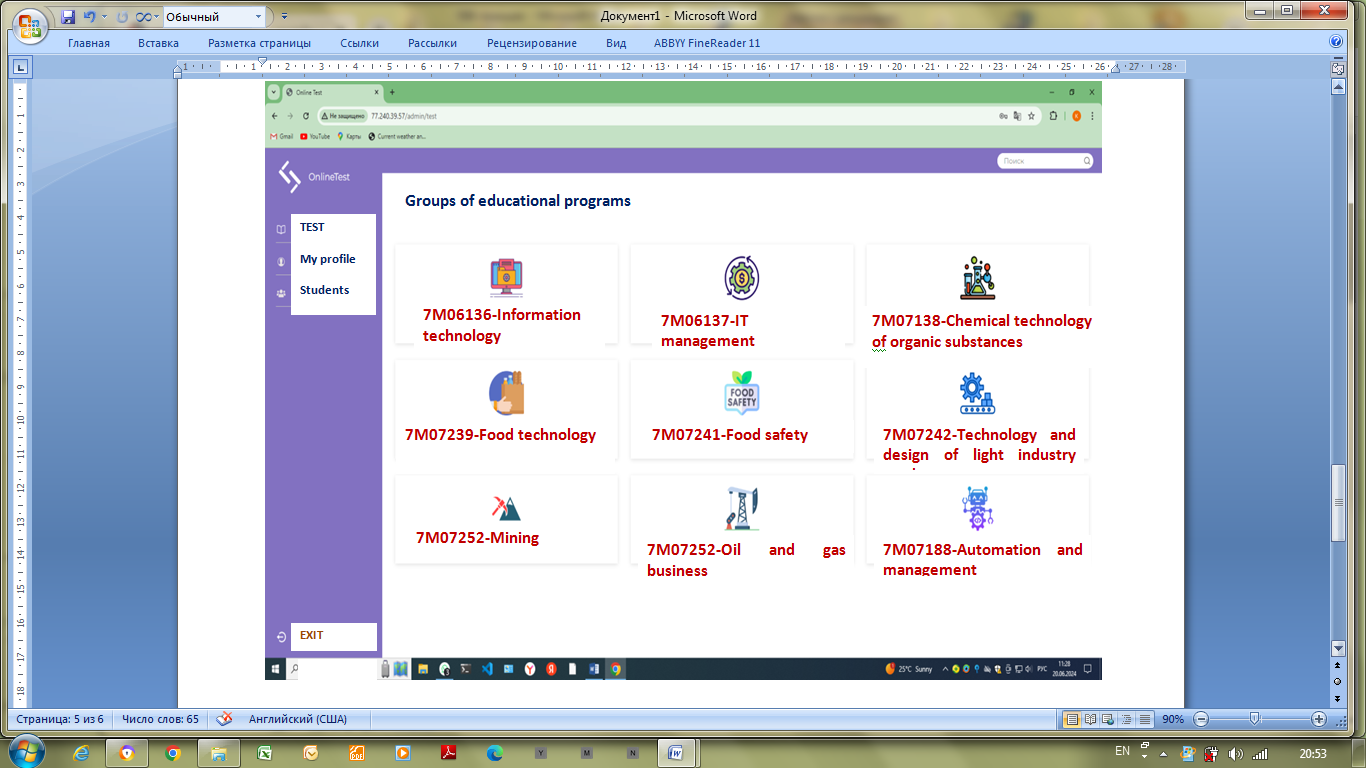
\includegraphics[width=0.8\textwidth]{assets/132}
	\caption*{\bfseries Figure 7−The main menu of the program code "Assistant for
	preparing test tasks"}
\end{figure}

\begin{multicols}{2}

Each educational program contains disciplines in which the student is
tested fig.8.
\end{multicols}

\begin{figure}[H]
	\centering
	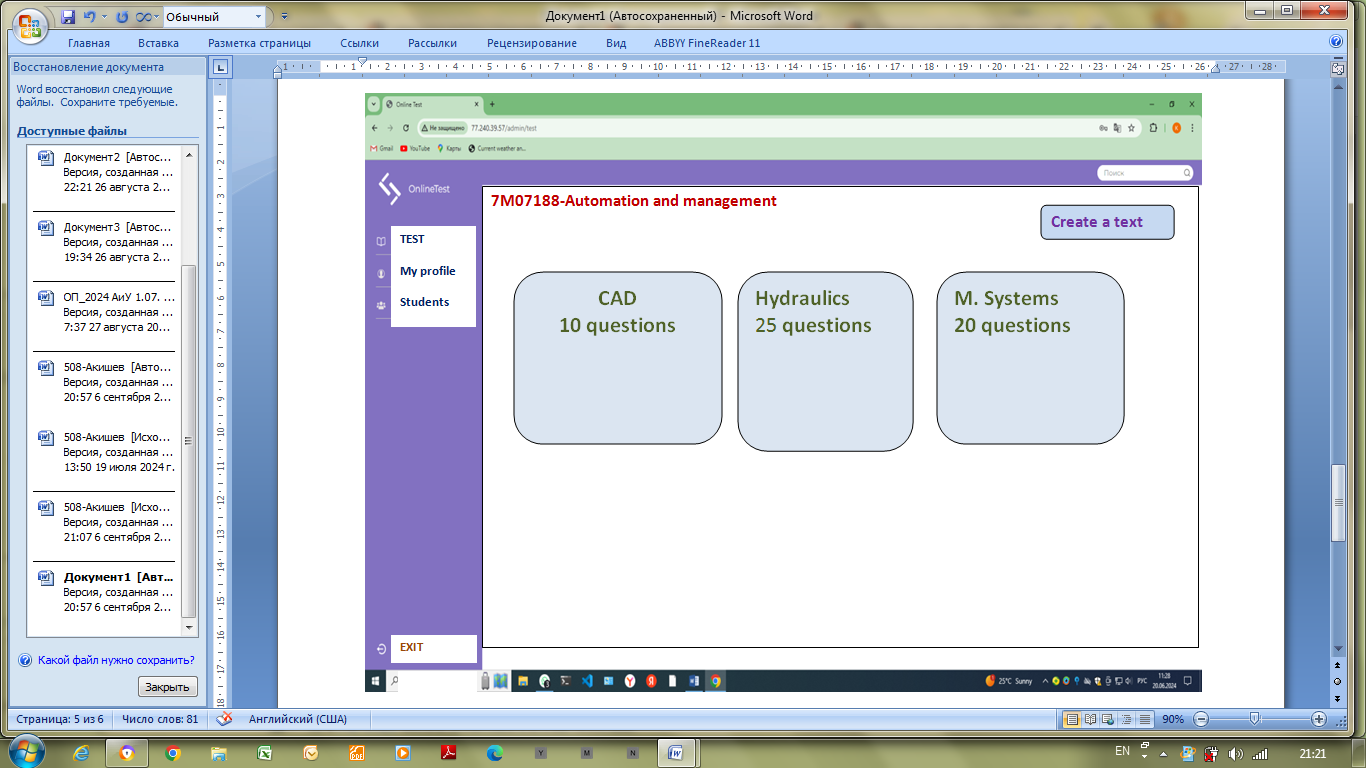
\includegraphics[width=0.8\textwidth]{assets/133}
	\caption*{\bfseries Figure 8−An example of disciplines for testing students}
\end{figure}



\begin{multicols}{2}
The development of tests begins with entering the name of the discipline
(in our example, the subject "Controller Programming" for the
educational program is Automation and control), the number of test
questions, and the time to answer fig.9.
\end{multicols}

\begin{figure}[H]
	\centering
	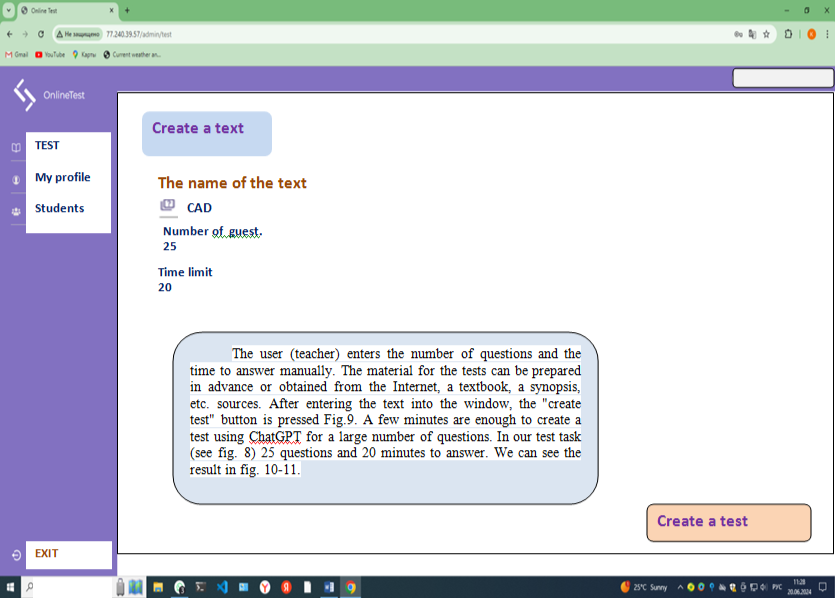
\includegraphics[width=0.8\textwidth]{assets/134}
	\caption*{\bfseries Figure 9−Development of test tasks}
\end{figure}

\begin{multicols}{2}

The user (teacher) enters the number of questions and the time to answer
manually. The material for the tests can be prepared in advance or
obtained from the Internet, a textbook, a synopsis, etc. sources. After
entering the text into the window, the "create test" button is pressed
Fig.9. A few minutes are enough to create a test using ChatGPT for a
large number of questions. In our test task (see fig. 8) 25 questions
and 20 minutes to answer. We can see the result in fig. 10-11.
\end{multicols}



\begin{figure}[H]
	\centering
	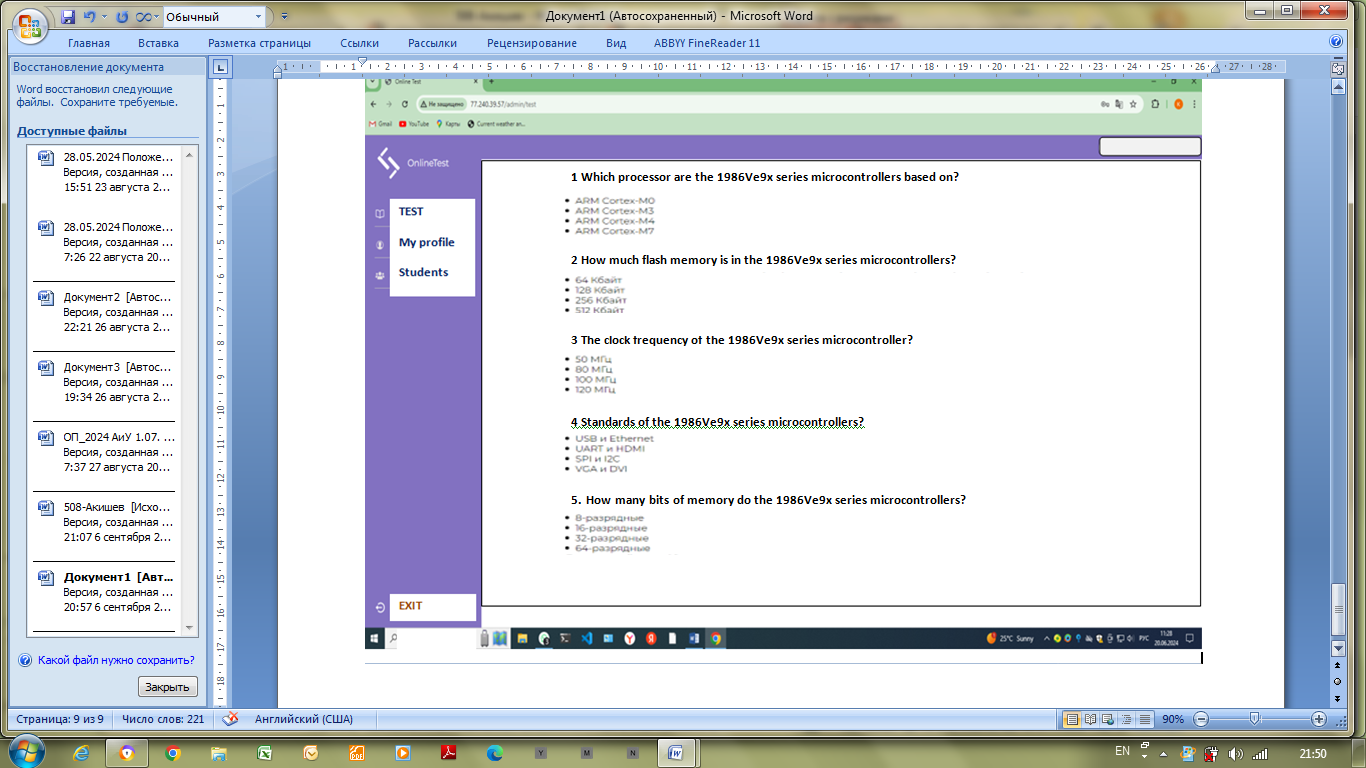
\includegraphics[width=0.8\textwidth]{assets/135}
	\caption*{\bfseries Figure 10− Developed test questions from 1-6}
\end{figure}


\begin{figure}[H]
	\centering
	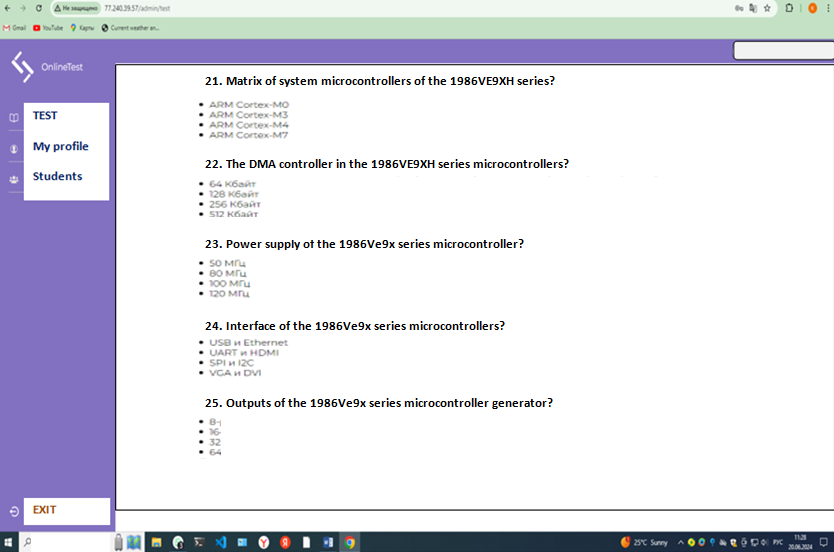
\includegraphics[width=0.8\textwidth]{assets/136}
	\caption*{\bfseries Figure 11− Developed test questions from 20-25}
\end{figure}

\begin{multicols}{2}
The resulting test is automatically placed in the Educational Programs
automation and Management folder fig.12.
\end{multicols}

\begin{figure}[H]
	\centering
	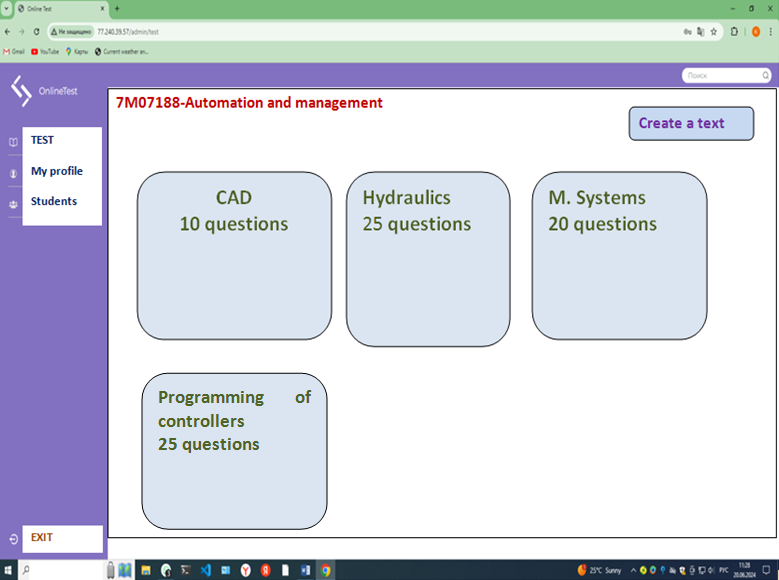
\includegraphics[width=0.8\textwidth]{assets/137}
	\caption*{\bfseries Figure 12- Developed test on the discipline "Controller
	programming"}
\end{figure}

\begin{multicols}{2}

Students of the groups are added to the appropriate discipline to
complete the test tasks fig.13, this requires their login and email in
gmail.com.
\end{multicols}


\begin{figure}[H]
	\centering
	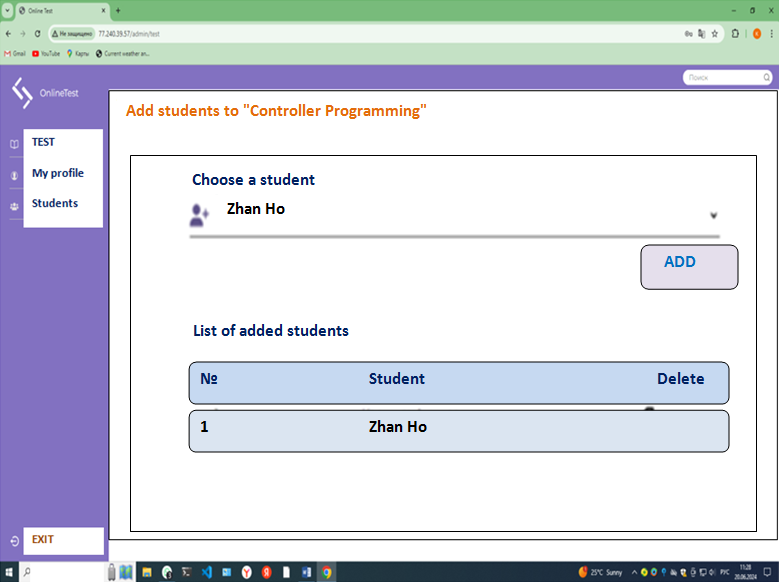
\includegraphics[width=0.8\textwidth]{assets/138}
	\caption*{\bfseries Figure 13−Adding students to control knowledge}
\end{figure}

\begin{multicols}{2}

After the registration of a student, he can take a test to check his
knowledge of the disciplines of the educational program in accordance
with the curriculum.

Fig. 14 shows the answer to the test tasks in the discipline "Controller
programming".
\end{multicols}


\begin{figure}[H]
	\centering
	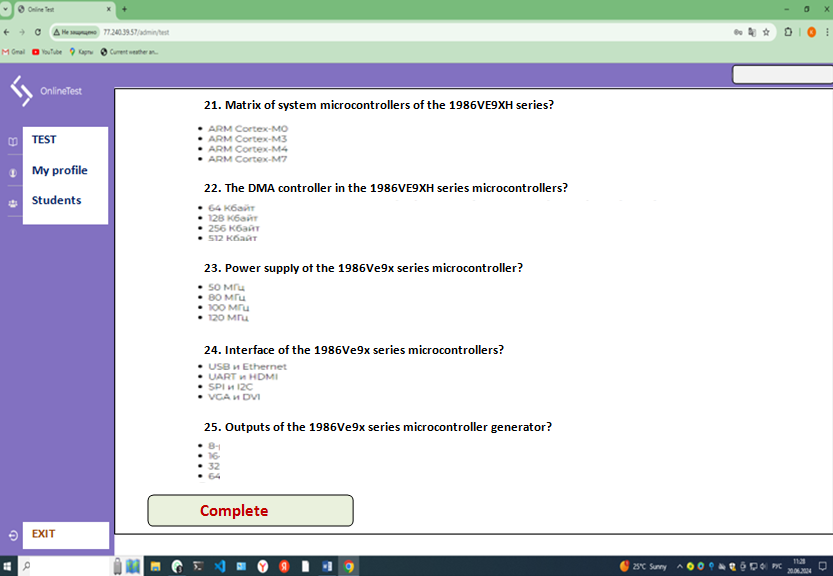
\includegraphics[width=0.8\textwidth]{assets/139}
	\caption*{\bfseries Figure 14- Completing the answers to the test}
\end{figure}


The result of the response can be viewed in a separate folder fig.15.

\begin{figure}[H]
	\centering
	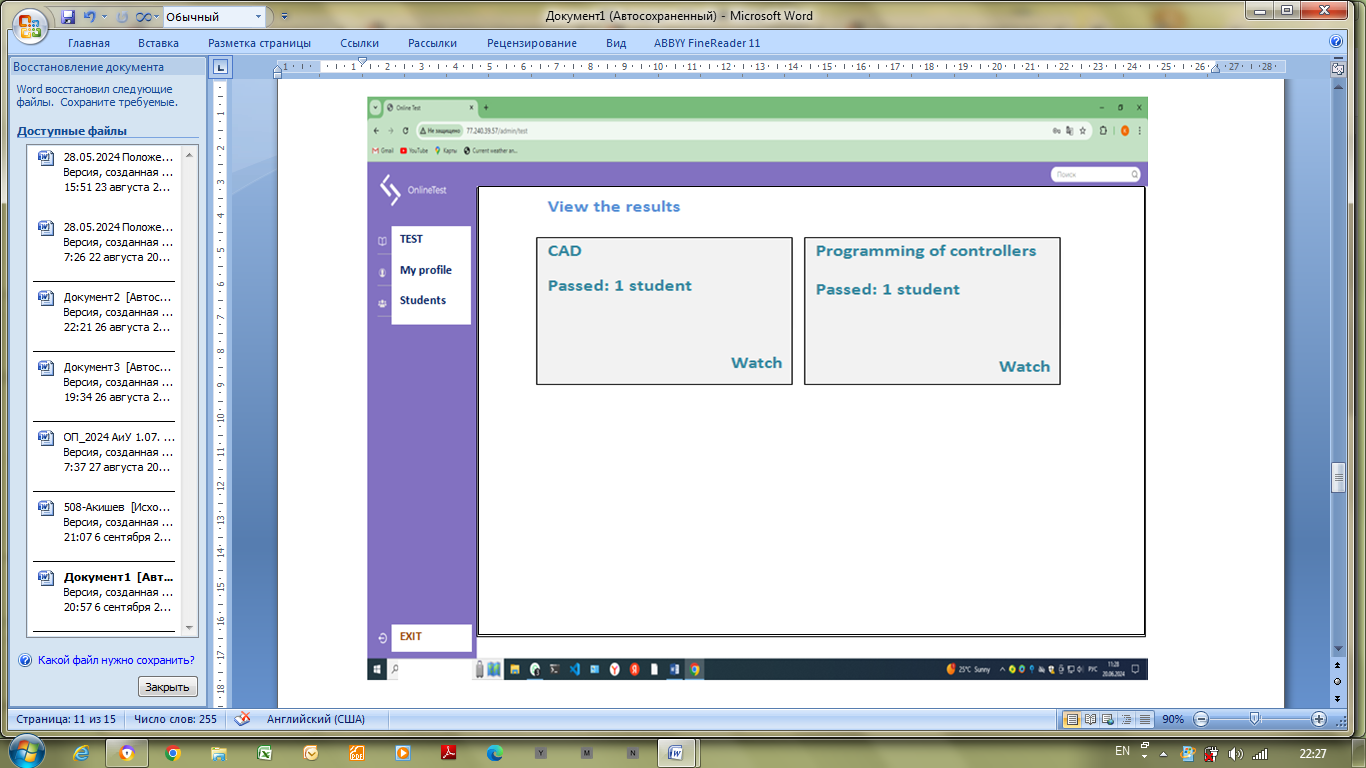
\includegraphics[width=0.8\textwidth]{assets/140}
	\caption*{\bfseries Figure 15−Storage location for students\textquotesingle{}
	answers}
\end{figure}


\begin{multicols}{2}
The result of the answer is given as a percentage of the equivalent
number of points received by students fig.16.
\end{multicols}

\begin{figure}[H]
	\centering
	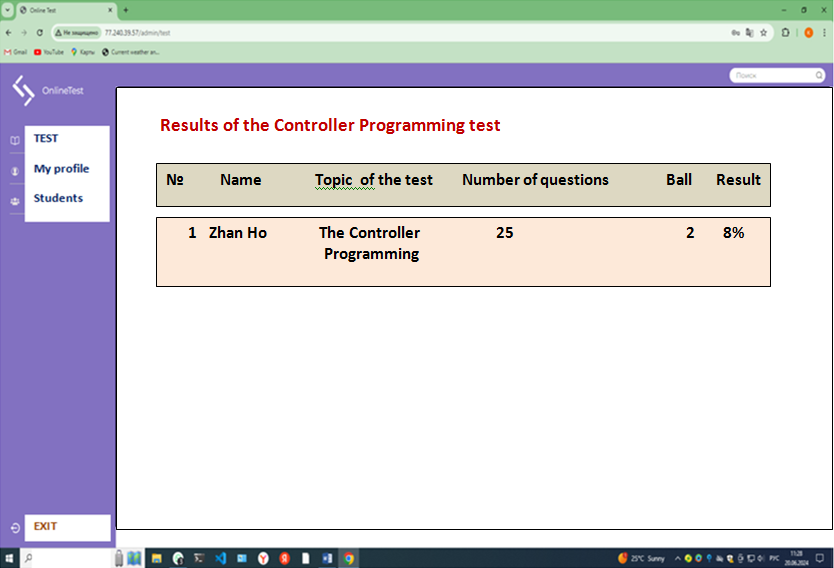
\includegraphics[width=0.8\textwidth]{assets/141}
	\caption*{\bfseries Figure 16−The result of the student\textquotesingle s answer to
	the test questions}
\end{figure}

\begin{multicols}{2}
Currently, the program code does not generate graphical tasks, and it
does not have the possibility of randomization, since these tasks were
not set for research purposes.

{\bfseries Conclusion.} The developed computer program "Assistant for the
preparation of test tasks" allows you to automate the process of
preparing test tasks for text of any volume and number of questions;

The program code can be used in educational institutions of the Ministry
of Education and the Ministry of Science and Higher Education of the
Republic of Kazakhstan and does not require high-performance computers
and a large amount of memory.

The practical application of the developed program "Assistant for the
preparation of test tasks" allows to increase the effectiveness of the
teacher\textquotesingle s work by 80\% compared to existing analogues
for the development of test tasks. At the same time, the quality and
adequacy of the developed issues are at a high level.
\end{multicols}


\begin{center}
	{\bfseries References}
\end{center}
\begin{noparindent}

1. Zakon Respubliki Kazakhstan. O vnesenii izmenenii I dopolnenii v
netkotorie zakonodatel'nie akti Respubliki Kazakhstan po voprosam
stimulirovaniya innovacii, razvitiya cifrovizacii, informacionnoi
bezopasnosti i obrazovaniya. Rasporyazhenie Prem'er ministra RK ot 25
avgusta 2022 goda № 128-r. URL:https://online.zakon.kz/ Document/
?doc\_id=33516174. {[}in Russ.{]}

2.Nestik T.A. ,Zhuravlev A.L. Social'no psikhologicheskaya determinaciya
gotovnostilichnosti k ispolzovaniu novikh tekhnologii
{[}Socio-psychological determination of a person\textquotesingle s
readiness to use new technologies// Psychological Journal.-
2018.-Т.39(5). -С. 5-14. DOI 10.31857/S020595920000829-7 {[}in Russ.{]}

3.Brazdil, P., Jorge, A. Progress in Artificial Intelligence: Knowledge
Extraction, Multi-Agent Systems, Logic Programming, and Constraint
Solving; Springer: Berlin/Heidelberg, Germany, 2001.-418P. ISBN
9783540430308

4.M. Montenegro-Rueda{\bfseries ,}J. Fernández-Cerero{\bfseries ,}José M.
Fernández-Batanero, E. López-Meneses. Impact of the Implementation of
ChatGPT in Education: A Systematic Review.//Computers.-\emph{~}2023.-
Vol.12(8).- P. 153.-P.1-13. \\~DOI 10.3390/computers12080153

5.García-Peña, V.R.; Mora-Marcillo, A.B.; Ávila-Ramírez, J.A. La
inteligencia artificial en la educación// Domino De Las Cienc.
-2020.-Vol. 6 (3).- P. 648-666. DOI 10.23857/dc.v6i3.1421

6. Incio Flores, F.A., Capuñay Sánchez, D.L., Estela Urbina, R.O.,
Valles Coral, M.A., Vergara Medrano, S.E.,EleraGonzáles, D.G.
Inteligencia artificial eneducación: Unarevisión de la literatura en
revistas científicas internacionales// \\Revista de Investigación Apuntes
Universitarios. - ~2022.-Vol. 12(1)- P.353-372. DOI
10.17162/au.v12i1.974

7. Neuman, M.; Rauschenberger, M.; Schön, E.M. We Need To Talk About
ChatGPT:\\The Future of AI and Higher Education//Hochschule
Hannover.-2023.- P.1-4. DOI 10.25968/opus-2467

8. García Sánchez, O.V. Uso y Percepción de ChatGPTen la Educación
Superior// RITI Journal

-2023.- Vol. 11(23).- P.98-107. DOI 10.36825/RITI.11.23.009

9. Osorio, J.A.C. Explorando el potencial de ChatGPTen la
escrituracientífica: Ventajas, desafíos y precauciones// Sci. Et
Tech.-2023.-Vol.28(01).- P.3-5.DOI 10.22517/23447214.25303

10. Qadir, J. Engineering Education in the Era of ChatGPT: Promises and
Pitfalls of Generative AI for Education//IEEE Global Engineering
Education Conference (EDUCON).- 2023.

DOI 10.1109/EDUCON54358.2023.10125121

11. Wang T., Lund B.D., Marengo A., Pagano A., Mannuru N.R., Teel Z.A.,
Pange J. Exploring the Potential Impact of ArtificialIntelligence (AI)
on International Students in Higher Education: Generative AI, Chatbots,
Analytics, and International Student Success// Appl.Sci -2023. -Vol. 13,
6716. DOI 10.20944/preprints202305.0808.v1

12. García-Peñalvo, F.J. La percepción de la Inteligencia Artificial
encontextoseducativostras el lanzamiento de ChatGPT: Disrupcióno pánico
// Educ. Knowl. Soc. (EKS). -2023.-Vol 24, e31279. DOI
10.14201/eks.31279

13 Аkishev K. Computer program "Assistant for the preparation of test
tasks. Certificate of entry of information into the State register of
rights to copyrighted objects No. 48275 dated July 10, 2024. NIISRK.
\end{noparindent}


\emph{{\bfseries Information about the authors}}
\begin{noparindent}

Akishev K. M. - Candidate of Technical Sciences, Ass. Professor, Kazakh
University of Technology and Business named after K. Kulazhanov, Astana,
Kazakhstan, e -mail:akmail04cx@mail.ru;

Tulegulov A. D.- Candidate of physics and mathematics Sciences, Ass.
Professor, Kazakh University of Technology and Business named after. K.
Kulazhanov,Astana, Kazakhstan,e-mail:tud62@yandex.ru;

Zhamangarin D. S.- Ph.D., Ass. Professor, Kazakh University of
Technology and Business named after. K. Kulazhanov, Astana, Kazakhstan
e-mail:dus\_man89@mail.ru;

Nurtai Z.T. - Ph.D., Ass. Professor, Kazakh University of Technology and
Business named after. K. Kulazhanov,Astana, Kazakhstan, e-mail:
zhadira\_nurtai@mail.ru;

Ospanov E. А.- PhD, Associate Professor,NAO Shakarim University, Semey,
Kazakhstan, e -mail:78oea@mail.ru;
\end{noparindent}

\emph{{\bfseries Информация об авторах}}
\begin{noparindent}
Акишев К. М. -к.т.н., асс. профессор, Казахский университет технологии и
бизнеса \\им. К. Кулажанова,Астана, Казахстан,e-mail:akmail04cx@mail.ru;

Тулегулов А. Д.- к.ф.м.н., асс. профессор, Казахский университет
технологии и бизнеса им. К. Кулажанова,Астана, Казахстан:
e-mail:tud62@yandex.ru;

Жамангарин Д. С.- доктор PhD , асс. профессор Казахский университет
технологии и бизнеса им. К. Кулажанова, Астана,
Казахстан,e-mail:dus\_man89@mail.ru;

Нуртай Ж.Т. - доктор PhD, асс. профессор, Казахский университет
технологии и бизнеса им. К. Кулажанова,

Астана, Казахстан, e-mail: zhadira\_nurtai@mail.ru;

Оспанов Е. А.- доктор PhD, асс. профессор, НАО «Университет имени
Шакарима, Семей, Казахстан, \\e-mail:78oea@mail.ru
\end{noparindent}
